\documentclass[slide,papersize]{jsarticle}
\usepackage[dvipdfmx]{graphicx,color}
\begin{document}

\section*{Activity と Intent}
\vspace*{8mm}
\begin{center}
{\Huge {\bf Activity\\と\\Intent}}
\end{center}

\section*{Activity と Intent}
\bigskip
\begin{itemize}
\item アプリケーションの構成要素
\bigskip
\item Activity の状態遷移
\bigskip
\item Intent
\end{itemize}

\section*{アプリケーションの構成要素}
\bigskip
\begin{itemize}
\item Activity
\bigskip
\item Broadcast Intent Receiver
\bigskip
\item Service
\bigskip
\item Content Provider
\end{itemize}

\section*{補足資料}
\bigskip
\begin{itemize}
%%\item http://www.cs.pitt.edu/\~{}tps9/anatomy.html
\item http://bit.ly/cYi4ed
\end{itemize}

\section*{Activity の状態遷移}
\medskip
\begin{center}
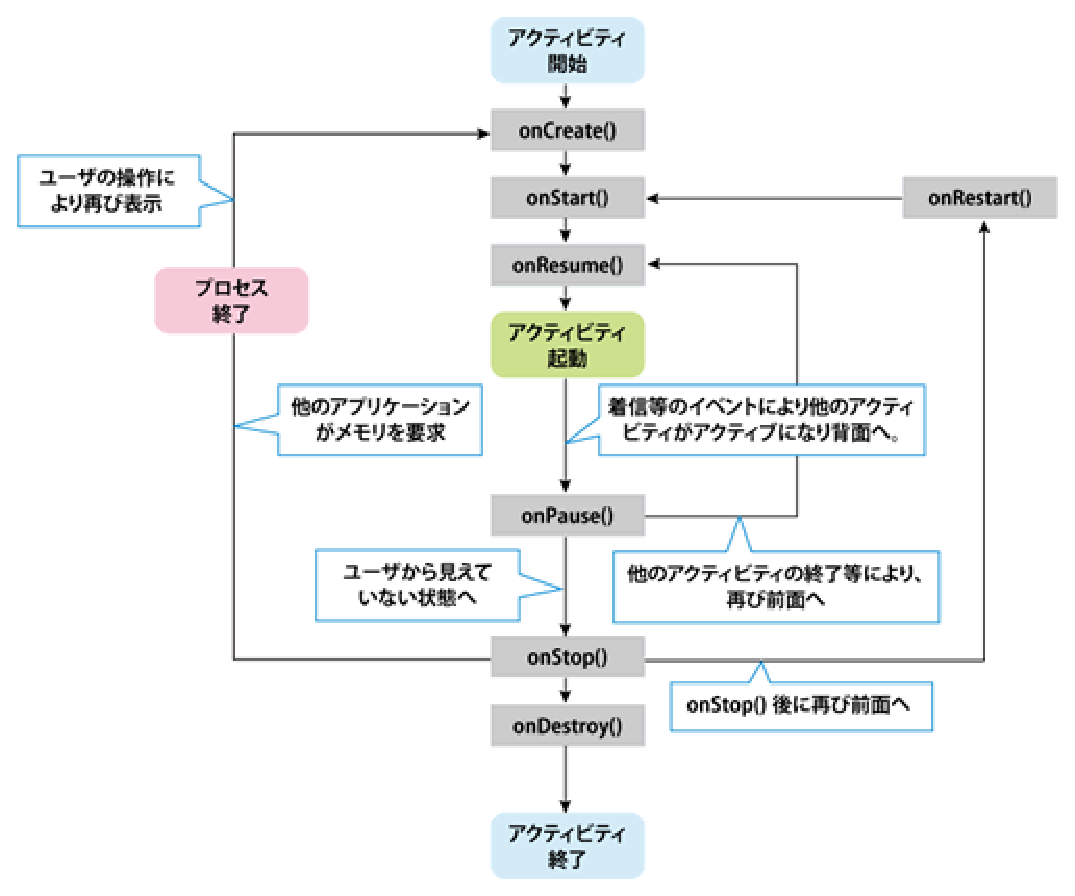
\includegraphics[scale=0.25]{ActivityLifecycle.eps}
\end{center}

\section*{動作確認}
\begin{itemize}
\item ハロワ作成
\item callback を定義して Log 出力させてみる
 \begin{itemize}
 \item {\footnotesize onCreate()}
 \item {\footnotesize onStart()}
 \item {\footnotesize onResume()}
 \item {\footnotesize onPause()}
 \item {\footnotesize onStop()}
 \item {\footnotesize onDestroy()}
 \end{itemize}
\item {\footnotesize 追加の方法は Source → Override/Implement Methods}
\end{itemize}

\section*{Intent}
Intent == 非同期メセジ
\medskip
\begin{center}
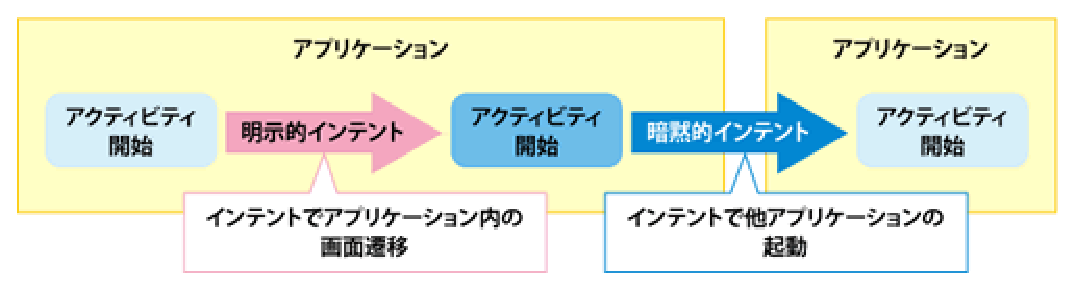
\includegraphics[scale=0.4]{Intent.eps}
\end{center}

\section*{画面遷移の例}
\bigskip
\begin{itemize}
\item 以下から download
 \begin{itemize}
 \item http://db.tt/zsaaZP
 \end{itemize}
\bigskip
\item Eclipse に import して確認
\bigskip
\item サブ画面を増やしてみましょう
\bigskip
\item Log 出力による動作確認とか
\end{itemize}

\section*{開発の基礎}
\bigskip
\begin{itemize}
\item http://bit.ly/KMrsQ
\end{itemize}

\end{document}
